\documentclass{article}
\usepackage[margin=1in]{geometry}
\usepackage[outdir=./]{epstopdf}  					% Avoids errors when input figures
\usepackage[labelsep=period,labelfont=bf]{caption}
%\usepackage{subcaption}
\usepackage{graphicx}
\usepackage{afterpage}

\begin{document}
	\afterpage{
	\begin{landscape}
	
	\begin{figure}[tbph]
		\caption{Response of the Yield Curve to a Target Surprise} \label{fig:LPEMtarget}
		\begin{center}
			\begin{minipage}{\linewidth}
				\begin{center}
					\begin{subfigure}[t]{\linewidth}
						\includegraphics[trim={0cm 0cm 0cm 0cm},clip,height=0.35\textheight,width=\linewidth]{../Figures/LPs/LagDep-FX/Target/EM/TargetEMnomyptpphi120m.eps} \\
						\vspace{-0.35cm}
						\caption{10-Year Yield} \label{subfig:LPEM10Ytarget}
						\vspace{0.4cm}
					\end{subfigure}
				
%					\vspace{0.5cm}
					
					\begin{subfigure}[t]{\linewidth}
						\includegraphics[trim={0cm 0cm 0cm 0cm},clip,height=0.35\textheight,width=\linewidth]{../Figures/LPs/LagDep-FX/Target/EM/TargetEMnomyptpphi24m.eps} \\
						\vspace{-0.35cm}
						\caption{2-Year Yield} \label{subfig:LPEM2Ytarget}
%						\vspace{0.4cm}
					\end{subfigure}
					\vspace{-0.45cm}
				\end{center}
				\fignotes{This figure shows the response following \cite{Jorda:2005} of the 10- and 2-year emerging market nominal yields and their components to a target easing surprise of 1 basis point. Nominal yields are decomposed into an expected future short-term interest rate, a term premium and credit risk compensation, see section \ref{sec:Decomposition} for details. Target surprises are identified using intraday data around Fed's monetary policy announcements, see section \ref{sec:USMPS} for details. An arrow indicates the contemporaneous (\(\idxh = 0\)) effect. The 90\% confidence bands are based on Driscoll--Kraay standard errors.}
			\end{minipage}
		\end{center}
	\end{figure}
	
	\pagebreak[4]
	
	\begin{figure}[tbph]
		\caption{Response of the Yield Curve to a Forward Guidance Surprise: 2000-2008} \label{fig:LPEMpathPre}
		\begin{center}
			\begin{minipage}{\linewidth}
				\begin{center}
					\begin{subfigure}[t]{\linewidth}
						\includegraphics[trim={0cm 0cm 0cm 0cm},clip,height=0.35\textheight,width=\linewidth]{../Figures/LPs/LagDep-FX/Path/EM/PathEMnomyptpphi120mPre.eps} \\
						\vspace{-0.35cm}
						\caption{10-Year Yield} \label{subfig:LPEM10YpathPre}
					\end{subfigure}
					
					\vspace{0.2cm}
					
					\begin{subfigure}[t]{\linewidth}
						\includegraphics[trim={0cm 0cm 0cm 0cm},clip,height=0.35\textheight,width=\linewidth]{../Figures/LPs/LagDep-FX/Path/EM/PathEMnomyptpphi24mPre.eps} \\
						\vspace{-0.35cm}
						\caption{2-Year Yield} \label{subfig:LPEM2YpathPre}
					\end{subfigure}
					\vspace{-0.45cm}
				\end{center}
				\fignotes{This figure shows the response following \cite{Jorda:2005} of the 10- and 2-year emerging market nominal yields and their components to a forward guidance easing surprise of 1 basis point. Nominal yields are decomposed into an expected future short-term interest rate, a term premium and credit risk compensation, see section \ref{sec:Decomposition} for details. Forward guidance surprises are identified using intraday data around Fed's monetary policy announcements, see section \ref{sec:USMPS} for details. An arrow indicates the contemporaneous (\(\idxh = 0\)) effect. The 90\% confidence bands are based on Driscoll--Kraay standard errors.}
			\end{minipage}
		\end{center}
	\end{figure}
	
	\pagebreak[4]
	
	\begin{figure}[tbph]
		\caption{Response of the Yield Curve to a Forward Guidance Surprise: 2008-2019} \label{fig:LPEMpathPost}
		\begin{center}
			\begin{minipage}{\linewidth}
				\begin{center}
					\begin{subfigure}[t]{\linewidth}
						\includegraphics[trim={0cm 0cm 0cm 0cm},clip,height=0.35\textheight,width=\linewidth]{../Figures/LPs/LagDep-FX/Path/EM/PathEMnomyptpphi120mPost.eps} \\
						\vspace{-0.35cm}
						\caption{10-Year Yield} \label{subfig:LPEM10YpathPost}
					\end{subfigure}
					
					\vspace{0.2cm}
					
					\begin{subfigure}[t]{\linewidth}
						\includegraphics[trim={0cm 0cm 0cm 0cm},clip,height=0.35\textheight,width=\linewidth]{../Figures/LPs/LagDep-FX/Path/EM/PathEMnomyptpphi24mPost.eps} \\
						\vspace{-0.35cm}
						\caption{2-Year Yield} \label{subfig:LPEM2YpathPost}
					\end{subfigure}
					\vspace{-0.45cm}
				\end{center}
				\fignotes{This figure shows the response following \cite{Jorda:2005} of the 10- and 2-year emerging market nominal yields and their components to a forward guidance easing surprise of 1 basis point. Nominal yields are decomposed into an expected future short-term interest rate, a term premium and credit risk compensation, see section \ref{sec:Decomposition} for details. Forward guidance surprises are identified using intraday data around Fed's monetary policy announcements, see section \ref{sec:USMPS} for details. An arrow indicates the contemporaneous (\(\idxh = 0\)) effect. The 90\% confidence bands are based on Driscoll--Kraay standard errors.}
			\end{minipage}
		\end{center}
	\end{figure}
	
	\pagebreak[4]
	
	\begin{figure}[tbph]
		\caption{Response of the Yield Curve to an Asset Purchase Surprise} \label{fig:LPEMlsap}
		\begin{center}
			\begin{minipage}{\linewidth}
				\begin{center}
					\begin{subfigure}[t]{\linewidth}
						\includegraphics[trim={0cm 0cm 0cm 0cm},clip,height=0.35\textheight,width=\linewidth]{../Figures/LPs/LagDep-FX/LSAP/EM/LSAPEMnomyptpphi120m.eps} \\
						\vspace{-0.35cm}
						\caption{10-Year Yield} \label{subfig:LPEM10Ylsap}
					\end{subfigure}
					
					\vspace{0.2cm}
					
					\begin{subfigure}[t]{\linewidth}
						\includegraphics[trim={0cm 0cm 0cm 0cm},clip,height=0.35\textheight,width=\linewidth]{../Figures/LPs/LagDep-FX/LSAP/EM/LSAPEMnomyptpphi24m.eps} \\
						\vspace{-0.35cm}
						\caption{2-Year Yield} \label{subfig:LPEM2Ylsap}
					\end{subfigure}
					\vspace{-0.45cm}
				\end{center}
				\fignotes{This figure shows the response following \cite{Jorda:2005} of the 10- and 2-year emerging market nominal yields and their components to an asset purchase easing surprise of 1 basis point. Nominal yields are decomposed into an expected future short-term interest rate, a term premium and credit risk compensation, see section \ref{sec:Decomposition} for details. Asset purchase surprises are identified using intraday data around Fed's monetary policy announcements, see section \ref{sec:USMPS} for details. An arrow indicates the contemporaneous (\(\idxh = 0\)) effect. The 90\% confidence bands are based on Driscoll--Kraay standard errors.}
			\end{minipage}
		\end{center}
	\end{figure}

	\end{landscape}
	}
\end{document}
% trim = {<left> <lower> <right> <upper>}